In this section we present the results of a series of experiments we have conducted using our EAGER prototype. We focus
on evaluating the overhead imposed by EAGER on the application deployment process as the number of deployed APIs and dependencies
grows. We also deploy a real-world API dataset (from ProgrammableWeb.com) on EAGER, and evaluate how a large 
volume of API metadata impacts EAGER.

\subsection{Experimental Control: Performance of AppScale without EAGER}

As a baseline, we start by analyzing how long it takes AppScale to deploy an
application.  The results are conservative in that they are taken from a
single VM deployment of AppScale (it is designed to run at scale) so that
logging and timing information would be easier to gather.  AppScale uses an
Ubuntu 12.04 Linux image which we hosted using Vagrant~\cite{XXXvagrantXXX}    
on a $2.7$ GHz x86 CPU with $4$ GB of memory.
Table~\ref{tab:sample_apps} lists a number of sample
applications along with their sizes and average deployment times on AppScale.
These applications represent a wide range of programming languages,
application sizes and business domains. The average deployment time is shown
for three runs each.

\begin{table}[ht]
\begin{center}
\begin{tabular}{| p{1.5cm} | p{3cm} | p{0.5cm} | p{1.1cm} | }
\hline
Application & Description & Size (MB) & Deployment Time (s) \\ \hline
guestbook-py & A simple Python web application that allows users to post
comments and view them & 0.16 & 22.13 \\ \hline
guestbook-java & A Java clone of the guestbook-python app & 52 & 24.18 \\ \hline
appinventor & A popular open source web application that enables creating mobile apps & 198 & 111.47 \\ \hline
coursebuilder & A popular open source web application used to facilitate teaching online courses & 37 & 23.75 \\ \hline
hawkeye & A sample Java application used to test AppScale & 35 & 23.37 \\ \hline
simple-jaxrs-app & A sample JAXRS app that exports 2 web APIs & 34 & 23.45 \\ \hline
dep-jaxrs-app & A sample JAXRS app that exports a web API and has one dependency & 34 & 23.72 \\ \hline
dep-jaxrs-app-v2 & A sample JAXRS app that exports 2 web APIs and has one dependency & 34 & 23.95 \\ \hline
\end{tabular}
\end{center}
\caption{Sample AppScale Applications}
\label{tab:sample_apps}
\end{table}

Note that the smallest deployment time recorded is $22.13$ seconds. Also 
there is
a clear correlation between the application size and the average deployment
time. Larger applications take longer to deploy because AppScale must transfer
the application code to servers as part of the deployment
process.  The experimental data represents the best possible scenario (in
terms of transfer latency) where the AppScale App Servers and the application
repository are located in the same VM.  At larger scale, the baseline
deployment times would likely be larger.

We noticed that the extra overhead imposed by EAGER is much smaller compared
to the overall application deployment times observed in the cloud (100's of
milliseconds compared to 10's of seconds).  Thus the first result is that
EAGER adds little overhead to the fastest deployment times we could achieve
with native AppScale.

To avoid confusion
caused by this scale difference and
improve the accuracy of our test results, we instrumented our experiments to
only record the extra time spent on EAGER. 
Hence, the figures that follow only present the additional time taken by EAGER
during application deployment process.  Note that the units for these
measurements of EAGER are one to two
orders of magnitude smaller than those for the
full deployment time.

\subsection{EAGER Overhead by Application}

Figure~\ref{fig:overhead_by_app} illustrates the time taken by EAGER to validate and verify the applications.
These results were recorded on an EAGER deployment without any policies deployed, and without any prior
metadata recorded in the API metadata manager (that is, on a clean database).

\begin{figure}
\centering
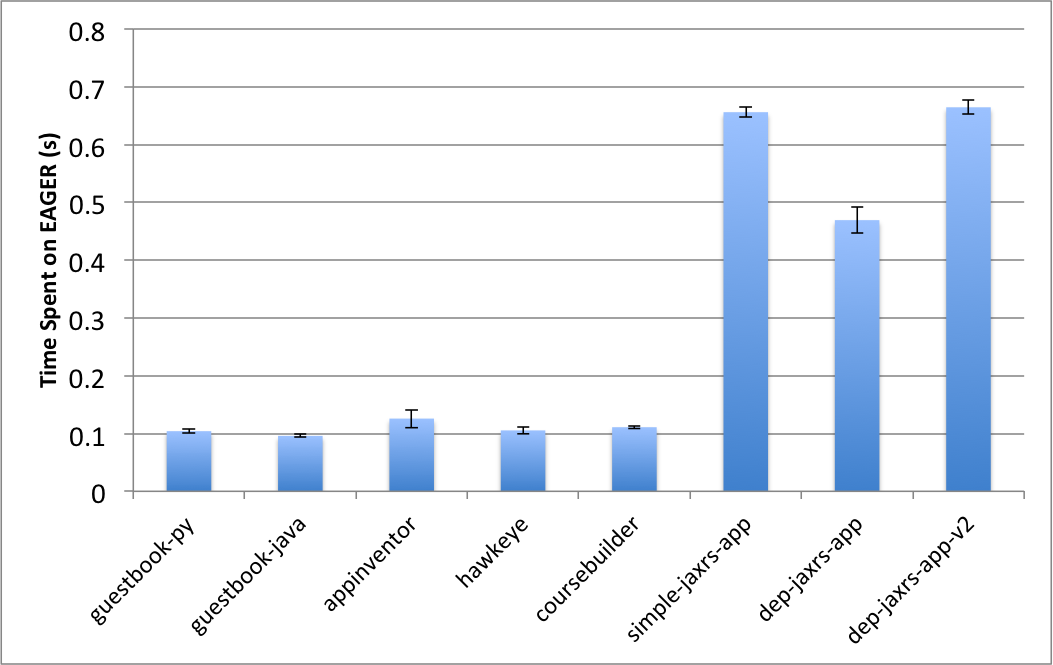
\includegraphics[scale=0.45]{overhead_by_app}
\caption{EAGER Overhead by Application}
\label{fig:overhead_by_app}
\end{figure}

Note that for the applications that do not export any web APIs, the overhead
is negligibly small (around 0.1s). This is because EAGER does not have to
contact the Metadata Manager for such applications. This implies that EAGER
will not affect the deployment time of most existing apps. For the
applications that export web APIs EAGER performs additional work. As a result
we see some extra overhead with such applications.  For applications that
export web APIs, the recorded overhead figures include the time it takes to
retrieve old API specifications from the Metadata Manager, the time it takes
to compare the new API specifications with the old ones, the time it takes to
update the API specifications and other metadata in the Metadata Manager and
the time it takes to publish the updated APIs to the cloud.  But even with
this extra work, the worst case observed overhead (for simple-jaxrs-app) is
$0.65s / 23.45s$ or 2.8\%.

%The overhead difference between dep-jaxrs-app and dep-jaxrs-app-v2 suggests that the EAGER overhead increases with the number
%of APIs exported by an application. In the next section we will further evaluate this difference.

\subsection{Impact of Number of APIs and Dependencies}

Figure~\ref{fig:overhead_by_apis} shows that the EAGER overhead grows linearly
with the number of APIs exported by an application.  This scaling occurs
because the current prototype implementation iterates through the APIs in the
application sequentially and records the API metadata in the Metadata Manager.
Then EAGER publishes each API to ADP and API Gateway. This sequencing
individual EAGER events, each of which generates a separate web service call,
represents an optimization opportunity in future implementations.
%additional web service calls, one per API. %Therefore, as more APIs are
%exported 
%by an application, the overhead of application deployment process via EAGER
%grows linearly. 

\begin{figure}
\centering
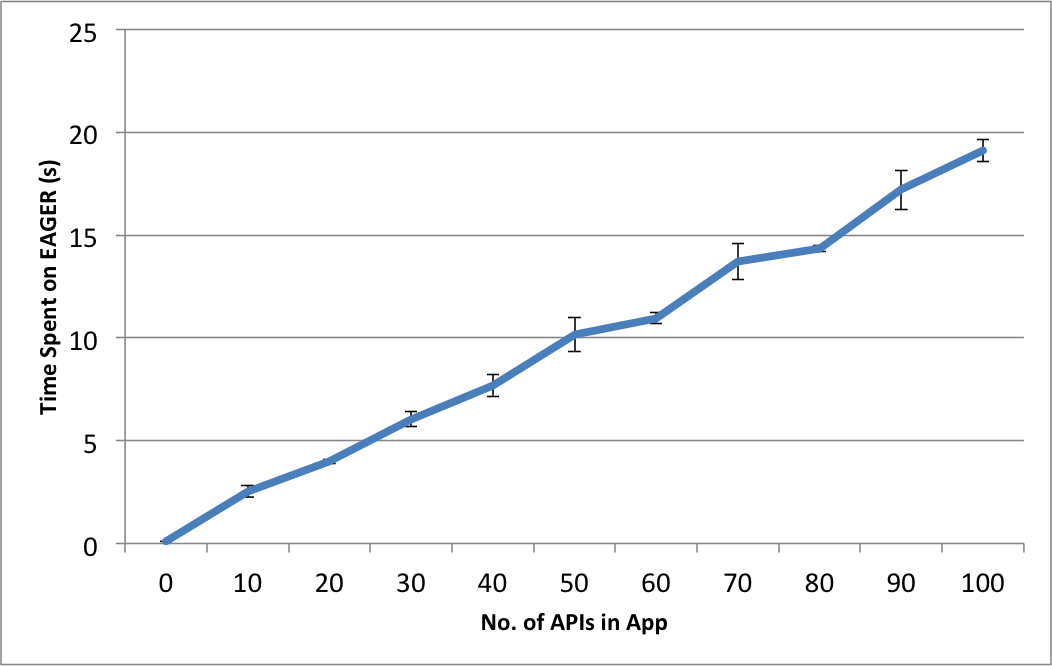
\includegraphics[scale=0.45]{overhead_by_apis}
\caption{EAGER Overhead vs. Number of APIs Exported by the Application}
\label{fig:overhead_by_apis}
\end{figure}

%We believe that in practice this linear growth in overhead is not significant to application developers.
However, at present, we expect 
most applications deployed in cloud to have a small to moderate number of 
APIs ($10$ or fewer).  With this API density EAGER's current scaling is
adequate.
%According to our results, this is an 
%extra overhead of 0.1-2.5 seconds. 
Even in the
unlikely case that a single application would export as many as $100$ APIs,
the total time for EAGER is under $20$ seconds.

%of 50 APIs being exported by an application, we can only see a percentage overhead around 30\%. 
%We can further improve the performance of EAGER by using multiple threads (one per API) to parallelize the API deployment process. %That is,
%%if the developer attempts to deploy an application that exports $n$ APIs, EAGER can spawn $n$ threads where each thread will be responsible
%for recording the metadata and publishing a single API.

Next, we analyze the EAGER overhead as the number of dependencies declared in
an application grows. For this experiment, we first populate the EAGER
Metadata Manager with metadata for $100$ randomly generated APIs. Then we
deploy an application on EAGER which exports a single API and declares
dependencies on the fictitious 
APIs that are already stored in the Metadata Manager. We
vary the number of declared dependencies and observe the EAGER overhead.

\begin{figure}
\centering
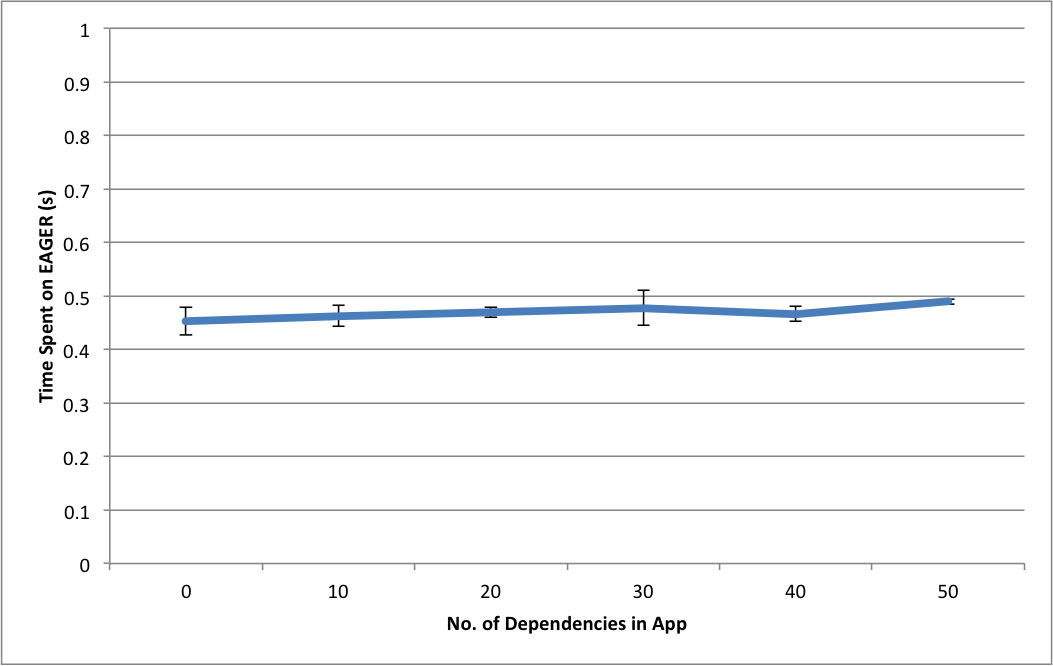
\includegraphics[scale=0.45]{overhead_by_deps}
\caption{EAGER Overhead vs. Number of Dependencies Declared in the Application}
\label{fig:overhead_by_deps}
\end{figure}

Figure~\ref{fig:overhead_by_deps} shows the results of this experiment. 
The EAGER overhead does not appear to be significantly
influenced by the number of dependencies declared in an application. 
IN this case, the EAGER implementation processes
all dependency-related information via batch operations. 
As a result, the number of web service calls and database queries that originate due to varying number of dependencies
is fairly constant. 
%This results in a reasonably constant overhead for the cases considered.

\subsection{Impact of Number of Policies}

So far we have conducted all our experiments without any active governance policies in the system. In this section we report how EAGER overhead
varies with the number of policies deployed in the PaaS. 

The overhead of policy validation is largely dependent on the actual policy
content (Python code). Since users may include any Python code they see fit
(as long as it falls in the accepted subset which prohibits aggregate
types and function calls) in a policy file, evaluating a
given policy could take an arbitrary amount of time (especially since
iteration is permitted). Therefore, in this
experiment, our goal is to evaluate the overhead incurred by simply having
many policy files to execute. We keep the content of the policies small and
trivial. We create a policy file that runs following assertions:
\begin{enumerate} 
\item Application name must start with an upper case letter
\item Application must be owned by a specific user 
\item All API names must start with upper case letters 
\end{enumerate} We create many copies of this
initial policy file to vary the number of policies deployed. Then we evaluate
the overhead of policy validation on two of our sample applications
(guestbook-py and simple-jaxrs-app). 

\begin{figure}
\centering
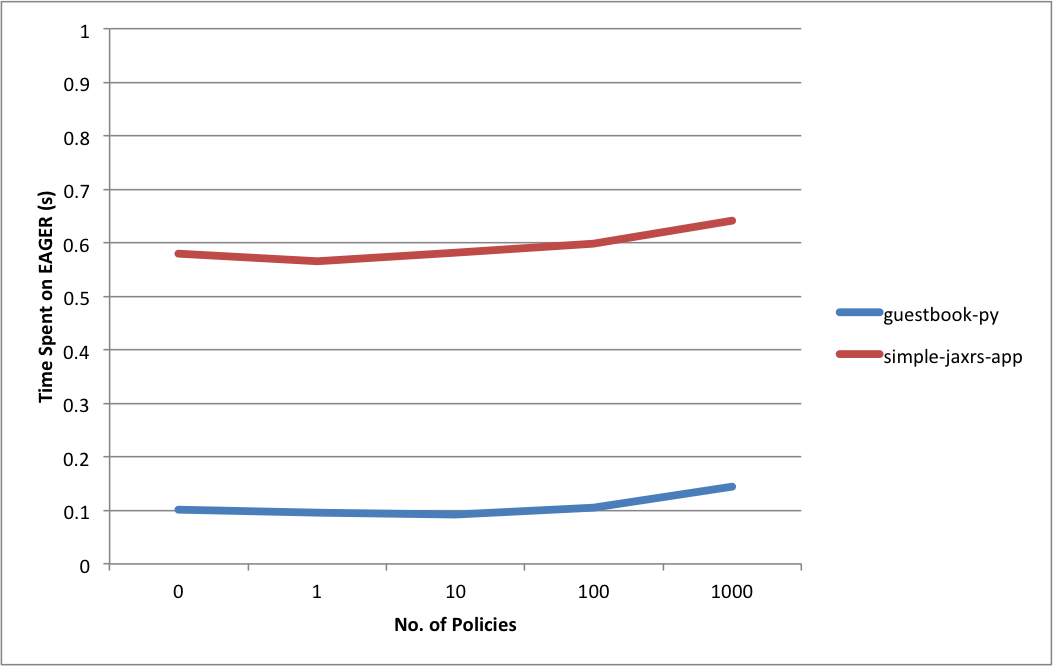
\includegraphics[scale=0.45]{overhead_by_policies}
\caption{EAGER Overhead vs. Number of Policies}
\label{fig:overhead_by_policies}
\end{figure}

Figure~\ref{fig:overhead_by_policies} shows how the number of active policies
impact the EAGER overhead. Interestingly, having many different policy files
have very little influence on the EAGER overhead. It is only when the active
policy count approaches $1000$ that we can see a noticeable increase in the
overhead. Even then, the increase in deployment time is under $0.1$ seconds. 

This is due to the fact that EAGER loads policy content into memory at system
startup (or when a new policy is deployed), and executes them from memory each
time an application is deployed. Since policy files are typically small (at
most a few kilobytes), this is a viable option. The overhead of validating the
simple-jaxrs-app is higher than that of the guestbook-py because,
simple-jaxrs-app exports web APIs. This means the third assertion in the
policy needs to be executed. 

Out results indicate that EAGER scales well to hundreds of policies. That is,
there is no significant overhead associated with simply having a large number
of policy files. However, as mentioned earlier, the content of a policy may
influence the overhead of policy validation.
 
\subsection{Scalability}
Next we evaluate how EAGER scales when a large number of APIs are deployed in the cloud. In this experiment, we populate the EAGER
Metadata Manager with a varying number of APIs, and then attempt to deploy various sample applications. We also create
random dependencies among the APIs recorded in the Metadata Manager to make the setting more realistic.

\begin{figure}
\centering
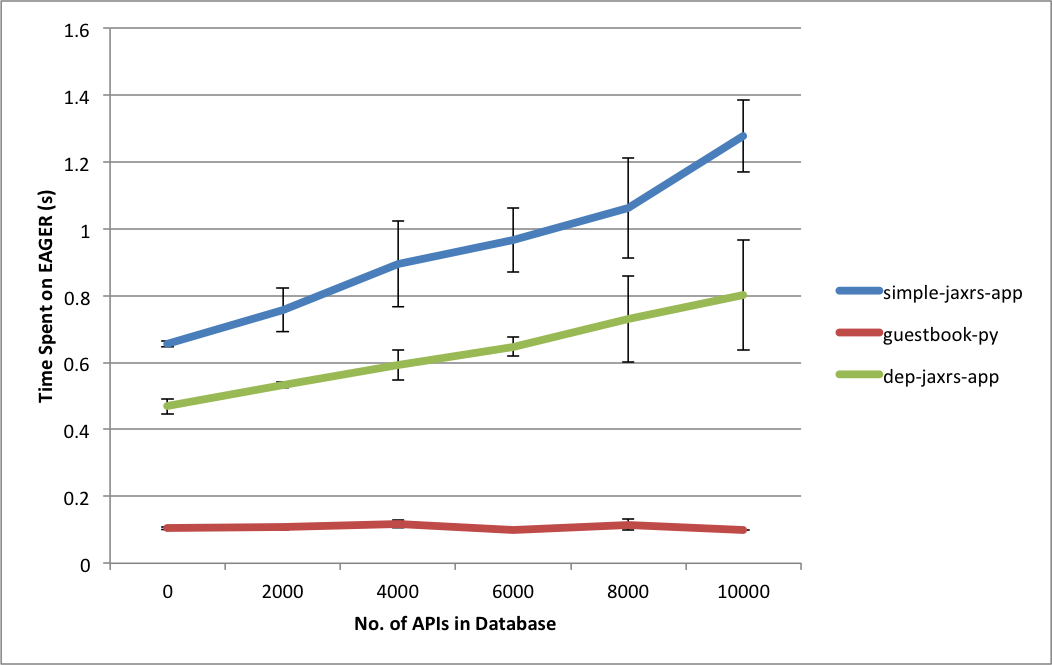
\includegraphics[scale=0.45]{scalability}
\caption{EAGER Overhead vs. Number of APIs in Metadata Manager}
\label{fig:scalability}
\end{figure}

Figure~\ref{fig:scalability} shows that the deployment overhead of the guestbook-py application is not impacted by the growth of metadata
in the cloud. Recall that guestbook-py does not export any APIs nor it declare any dependencies. Therefore the deployment process of
the guestbook-py application has minimal interactions with the Metadata Manager. Based on this result we conclude that applications that
do not export web APIs are not significantly affected by the accumulation of metadata in EAGER.

Both simple-jaxrs-app and dep-jaxrs-app are
somewhat affected by the volume of data stored in Metadata Manager. Since these applications export web APIs that must be 
recorded and validated by the Metadata Manager, the explosion of metadata has an increasingly higher impact on them. The degradation 
of performance is due to the slow query performance of the RDBMS engine (MySQL) as the database size grows. The simple-jaxrs-app
is affected more by this performance drop, because it exports two APIs compared to the single API exported 
by dep-jaxrs-app. However, the growth
in overhead is linear to the number of APIs deployed in the cloud. Also,
even after deploying $10000$ APIs, the overhead of simple-jaxrs-app has only been increased by about 0.5 seconds.

Another interesting attribute to notice in figure~\ref{fig:scalability} is the
growing amount of variance in the overhead as the number of APIs in the cloud
grows.  We believe this is due to the increasing variability of database query
performance and the data transfer performance as the size of the database
increases.

In summary, the current EAGER prototype scales well to $1000$'s of APIs.
%This is important given that popular API registries (e.g. ProgrammableWeb.com) 
%place the total number of APIs in the Internet somewhere in the range of 10000 to 15000. 
If further scalability is require in the future, it appears that there are
several opportunities for optimization.
%work from the database community, and use a faster, and more scalable database engine (e.g. NoSQL) to implement the
%EAGER Metadata Manager.

\subsection{Experimental Results with a Real-World Dataset}

Finally, we explore how EAGER operates with a real-world dataset with API
metadata and dependency information. For this, we crawl the ProgrammableWeb
registry and extract metadata regarding all the registered APIs and mashups.
At the time of the experiment, we collected $11095$ APIs and $7227$ 
mashups (each mashups depends on one or more APIs).

We populated the the EAGER Metadata Manager with all of the APIs and
registered each of the mashups as APIs in EAGER. We then used the
mashup-API dependency information to register dependencies among the APIs in 
EAGER. This resulted in a 
total dependency graph of $18322$ APIs with $33615$ dependencies. 
Then we deploy
some of our sample applications on EAGER to measure the overhead.

\begin{figure}
\centering
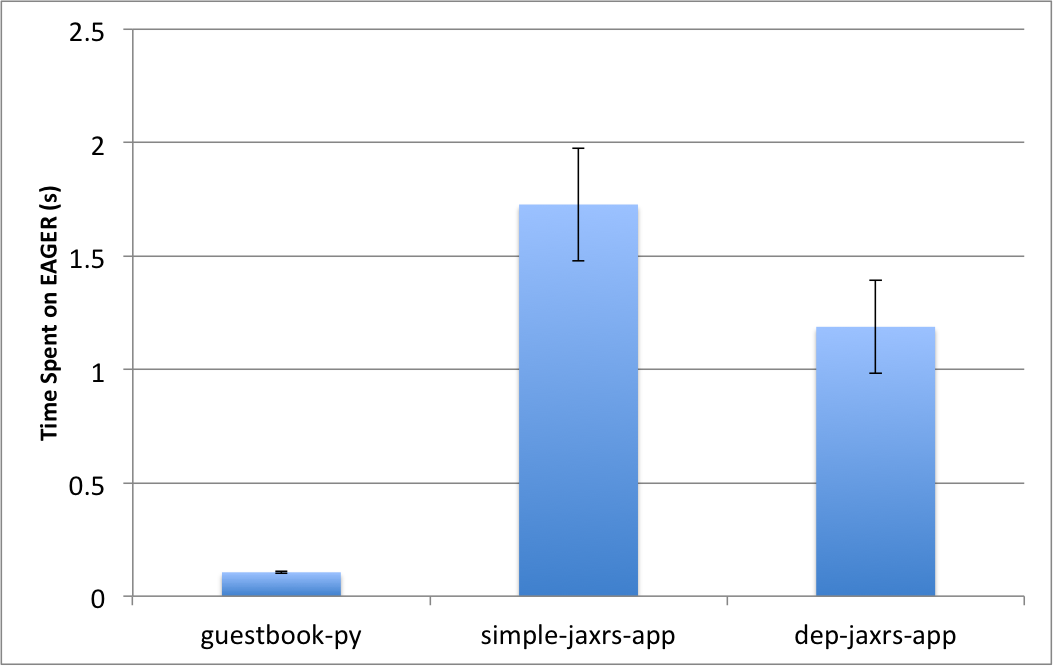
\includegraphics[scale=0.45]{pweb_sample_overhead}
\caption{EAGER Overhead When Deploying on ProgrammableWeb Dataset}
\label{fig:pweb_sample_overhead}
\end{figure}

As shown in figure~\ref{fig:pweb_sample_overhead}, the guestbook-py app is not
significantly impacted by the large dependency database. 
Recall that 
guestbook-py deploys and interacts with its users but doesn't export any 
web APIs.  Thus EAGER does not impact incident applications with no API
governance requirements. 
Applications that export web API show a slightly higher deployment overhead. 
But the highest overhead observed is under 2 seconds, which is still small 
compared
to the total application deployment time. 

All three sample applications considered in the above experiment do not declare dependencies on any of the APIs in the ProgrammableWeb
dataset. The dep-jaxrs-app does declare a dependency, but that is on an API exported by simple-jaxrs-app. To see how the deployment time is impacted
when applications take dependencies on other APIs registered in EAGER, we
deploy a test application that declares random fictitious dependencies on APIs
from the Programmable Web corpus registered in EAGER. 
We vary the declared dependency count randomly between $10$ and $50$ 
and also redeploy the application multiple times.
In one set of experiments (columns denoted with the prefix ``random'' in the
figure), we run a deployment script that randomly modifies the 
declared dependencies at each redeployment. In another set of 
experiments (denoted ``fixed''), we redeploy the application 
without randomizing the declared dependencies.

\begin{figure}
\centering
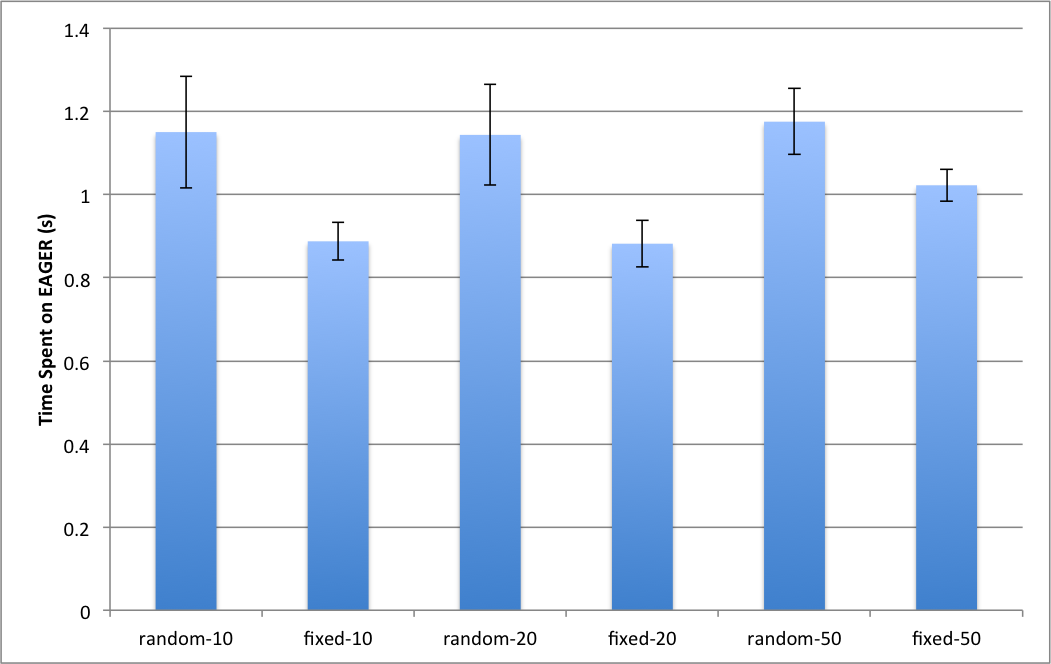
\includegraphics[scale=0.45]{pweb_random_overhead}
\caption{EAGER Overhead When Deploying on ProgrammableWeb Dataset with Dependencies}
\label{fig:pweb_random_overhead}
\end{figure}

%Figure~\ref{fig:pweb_random_overhead} illustrates results from both sets of
%experiments.  Columns labeled as ``random'' indicate the average overhead
%computed across 3 redeployments, where the declared dependencies were
%randomized prior to each redeployment. Columns labeled as ``fixed'' show the
%average overhead calculated across 3 redeployments, where the dependency
%declaration was kept fixed across redeployments. 
The numeric suffix to either ``random'' or ``fixed'' in each column
label indicates the number of dependencies declared.

Interestingly, dependency count does not have a significant impact on 
the overhead. %This is inline with our observations in figure~\ref{fig:overhead_by_deps}.
%It is encouraging to see that the same property holds when the Metadata Manager is loaded with over 18000 entries. 
The largest overhead observed is under 1.2 seconds.
Also whenever the dependency declaration was kept fixed, the overhead is slightly smaller. This is because our prototype caches
the edges of its internally generated dependency tree, 
which makes immediate redeployments go faster.

%Overall our experimental results indicate that EAGER can be successfully implemented in today's PaaS clouds, 
%with minimal modifications to the platform core.
Summarizing, 
EAGER adds very little overhead to the application deployment process, and the
overhead increases linearly with the number of APIs exported by the applications, and the number of APIs deployed in the cloud. 
Interestingly, the number of deployed policies and declared dependencies
have little impact on the EAGER governance overhead. Finally, our results indicate that EAGER scales
well to $1000$'s of APIs and adds no more than $2$ seconds with over
$18,000$ ``real-world''
deployed APIs in its database.
